%! Author = vojmo
%! Date = 29.01.2022

\chapter{Návrh}

\section{Vzhled aplikace}

Při navrhování aplikace se většinou začíná s takzvanými wireframy. Wireframe je rozložení prvků aplikace, které ještě
nemají žádný vzhled. Jsou to například tlačítka, sekce pro různý obsah atd. Já jsem zvolil lehce odlišný přístup, tedy
vytvoření wireframu již s designem. K této tvorbě jsem použil nástroj Adobe XD~\cite{AdobeXD}.

U vzhledu jsem se inspiroval moderními operačními systémy jako např. Windows 11~\cite{Windows11}, One UI~\cite{OneUI}
(nadstavba Android od společnosti Samsung) atd.
Chtěl jsem dosáhnout jednoduchého, přehledného designu, který bude pro uživatele příjemný na používání. Postupně jsem se
propracoval přes několik verzí a ve výsledku jsem zvolil průhledný styl podkladu komponent s \emph{mesh gradientem}~\cite{MeshGradients} na pozadí.

Již od počátku jsem bral v potaz rozdíly mezi zobrazením na mobilu a počítači, díky čemuž jsem mohl design uzpůsobit
pro více typů obrazovek. Začal jsem vytvářením úvodní obrazovky, na které se zobrazí rychlé odkazy na nejdůležitější části
aplikace, vyhledávání a logo. Tato stránka by měla být přehledná a čistá, proto jsem zvolil ikonky, které vystihují dané
odkazy. Díky tomu se při zobrazení na mobilu se tak mohou skrýt pomocné texty.

\begin{figure}[H]
    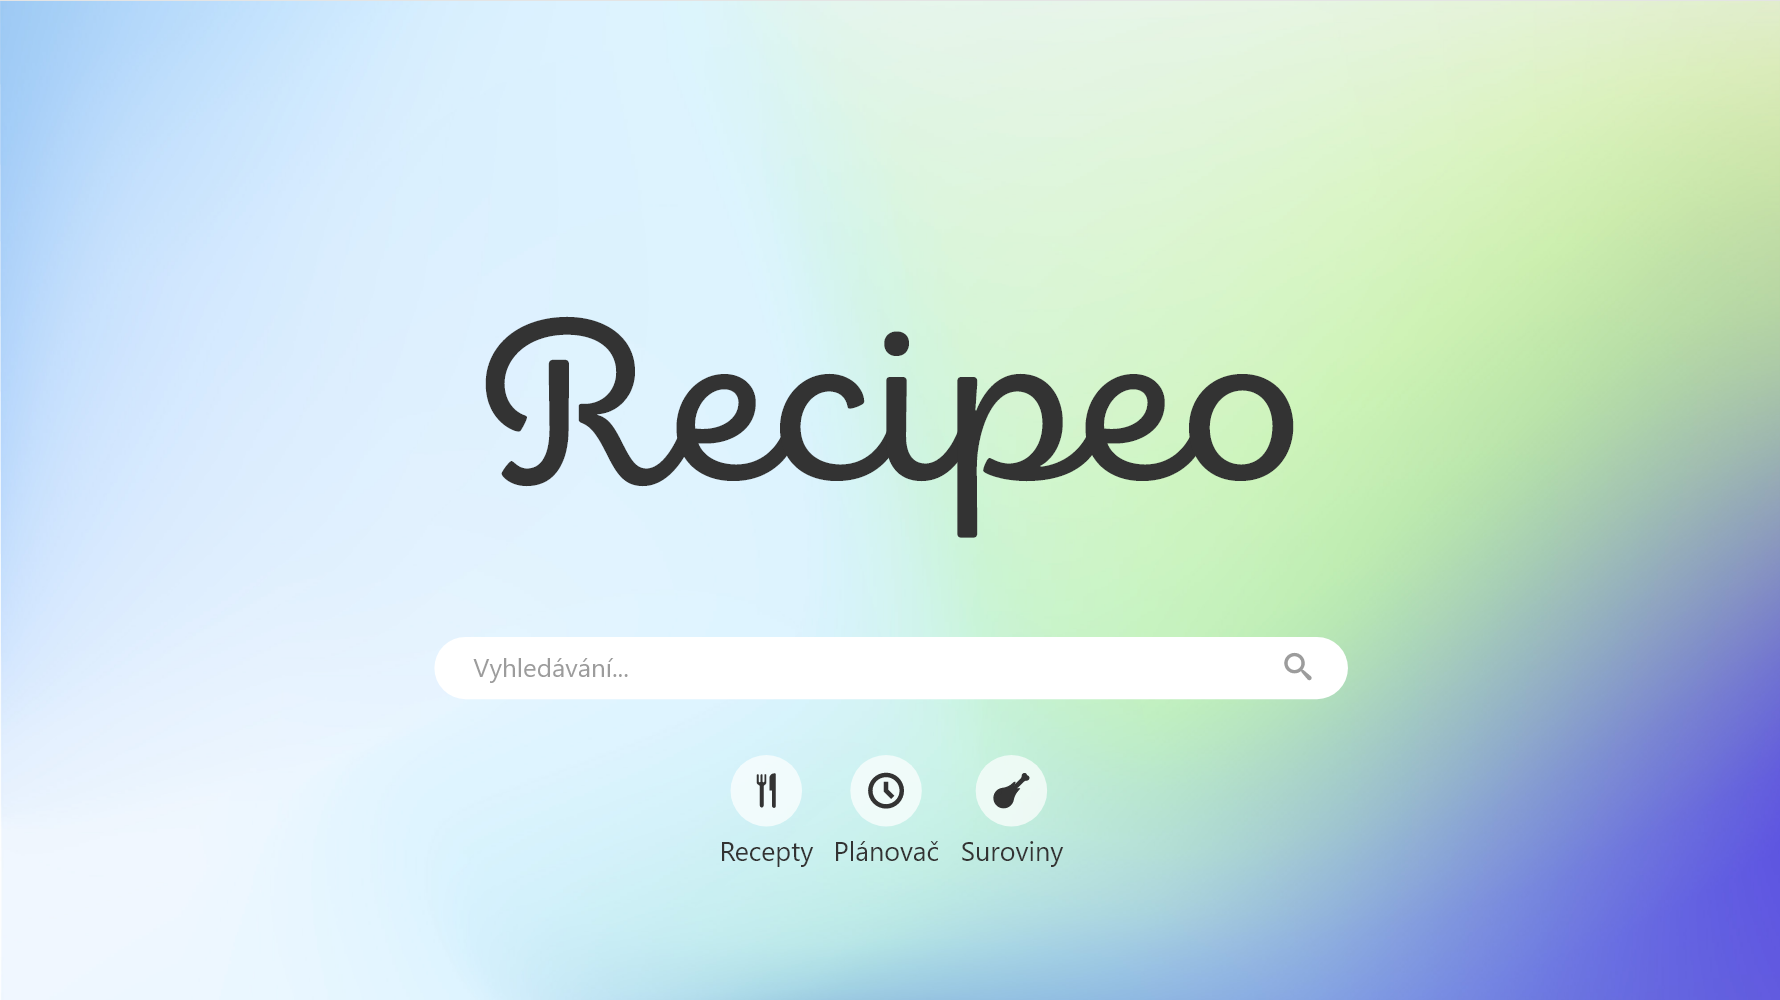
\includegraphics[width=\textwidth]{images/main-page}
    \caption{Hlavní obrazovka} \label{picture:recipeo:main-page}
\end{figure}

Dále jsem pokračoval se zobrazením receptů. Na verzi pro počítač jsem na levé straně umístil filtrování a zbylou plochu jsem ponechal
pro samotné recepty. Na menších obrazovkách se filtrování přesune nad seznam receptů a již nebude viditelné při posunutí směrem dolů.
Na \uv{karty} s recepty jsem vybral nejdůležitější informace. Tedy název, štítky a obrázek receptu. Nejprve jsem přidal do spodní části
karty i ozdobný motiv, později při implementaci jsme se ale s vedoucím dohodnuli, že pouze zabírá místo a bude lepší jej odebrat.

Zobrazení samotného receptu je na velkých a malých obrazovkách velmi odlišné. Zatímco na počítači se uživateli zobrazí všechny
informace v několika oddělených obdélnících, na mobilu se každá z těchto částí rozdělí na samostatnou záložku. Také se na spodku
obrazovky zobrazí lišta, pomocí které je možné záložky přepínat.

Seznam ingrediencí je stejný jako u receptů. Pro zobrazení ingredience platí totéž.

Plánovač jsem navrhnul jako kalendář, do kterého se dají přesunout recepty pomocí \emph{drag and drop}. Pro rychlý návrh receptu
jsem zvolil schéma podobné dnešním seznamkám. Tedy přijmutí popřípadě odmítnutí navrženého receptu je po stranách zobrazené karty
a vlevo ze nachází zásobník již zvolených receptů.

\section{Název a logo}
Pro aplikaci bylo potřeba vybrat název a logo. Vzhledem k tomu, že středem všeho jsou recepty, hrál jsem si s anglickým slovem
\emph{recipe}, až jsem se dostal na Recipeo. Tento název se líbil mně i vedoucímu, tak jsme zaregistrovali doménu \emph{www.recipeo.cz}.
Poté jsem založil nový soubor v Photoshopu a pustil se do vytváření loga. Chtěl jsem vytvořit jedno s celým názvem, které bychom použili
na úvodní stránce a jedno menší, které by se dalo využít jako ikona aplikace, favicon atd.

Zvolil jsem několik fontů z Adobe Fonts~\cite{AdobeFonts} a vytvořil návrhy. Menší logo jsem se rozhodl udělat jako první písmeno názvu na pozadí,
které se použije v aplikaci. Návrhů bylo celkem šest a na Slacku~\cite{Slack}, který jsme využívali pro komunikaci, jsme hlasovali, které je nejlepší.

\begin{figure}[h]
    \centering
    \subfloat[První návrh loga]{
\includegraphics[width=0.2\textwidth]{images/logo-1}\label{picture:recipeo:logo-1}}
    \hfill
    \subfloat[Druhý návrh loga]{
\includegraphics[width=0.2\textwidth]{images/logo-2}\label{picture:recipeo:logo-2}}
    \hfill
    \subfloat[Třetí návrh loga]{
\includegraphics[width=0.2\textwidth]{images/logo-3}\label{picture:recipeo:logo-3}}
    \hfill
    \subfloat[Výsledné logo]{
\includegraphics[width=0.2\textwidth]{images/logo-final}\label{picture:recipeo:logo-final}}
    \caption{Vývoj loga}
\end{figure}

\section{Databáze ve Firebase}
Jak jsem již zmínil, \emph{Firestore} je databáze ve službě \emph{Firebase}. Vytvořil jsem doménový model, který jsem ale poté musel přetransformoval pro
dokumentovou databázi.

\subsection{Doménový model}
% TODO: Přidat upravený obrázek
\begin{figure}[h]
    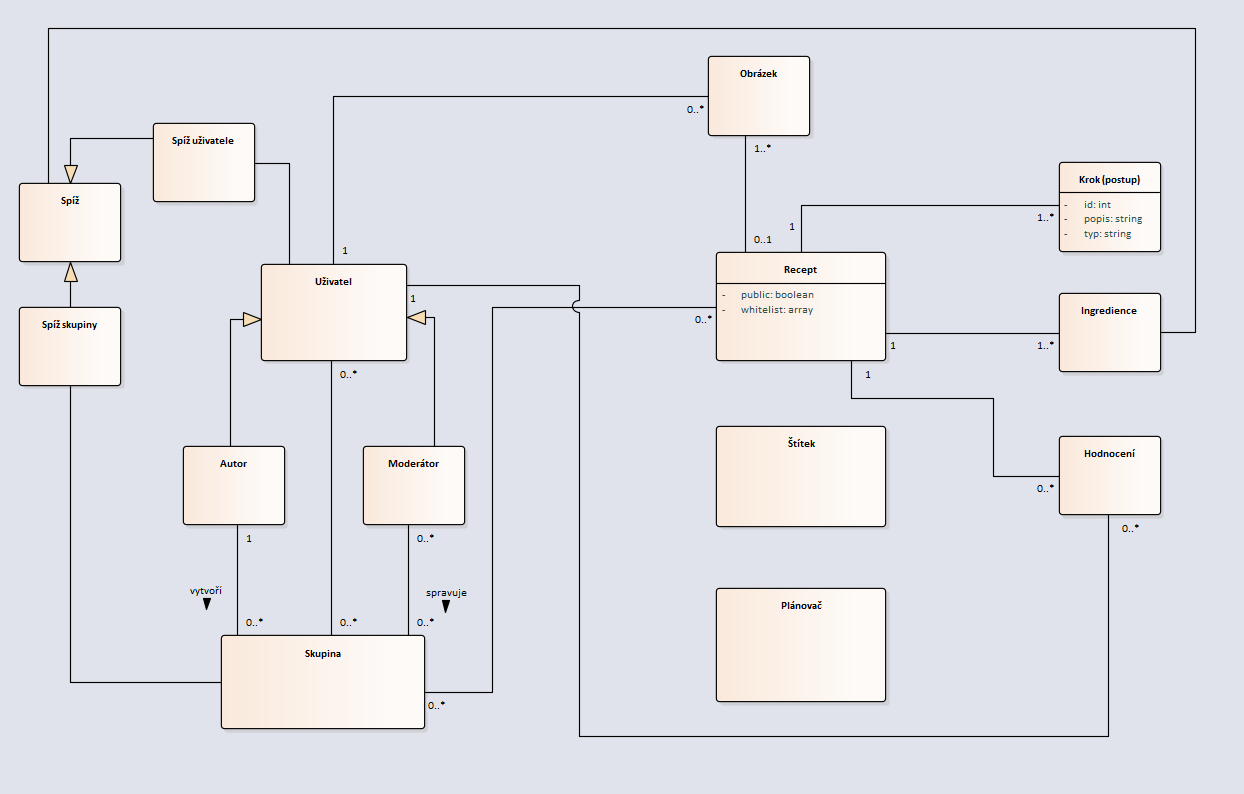
\includegraphics[width=\textwidth]{images/domain-model}
    \caption{Doménový model} \label{picture:recipeo:domain-model}
\end{figure}

\subsection{Schéma v dokumentové databázi}
% TODO: Přidat upravený obrázek
\begin{figure}[H]
    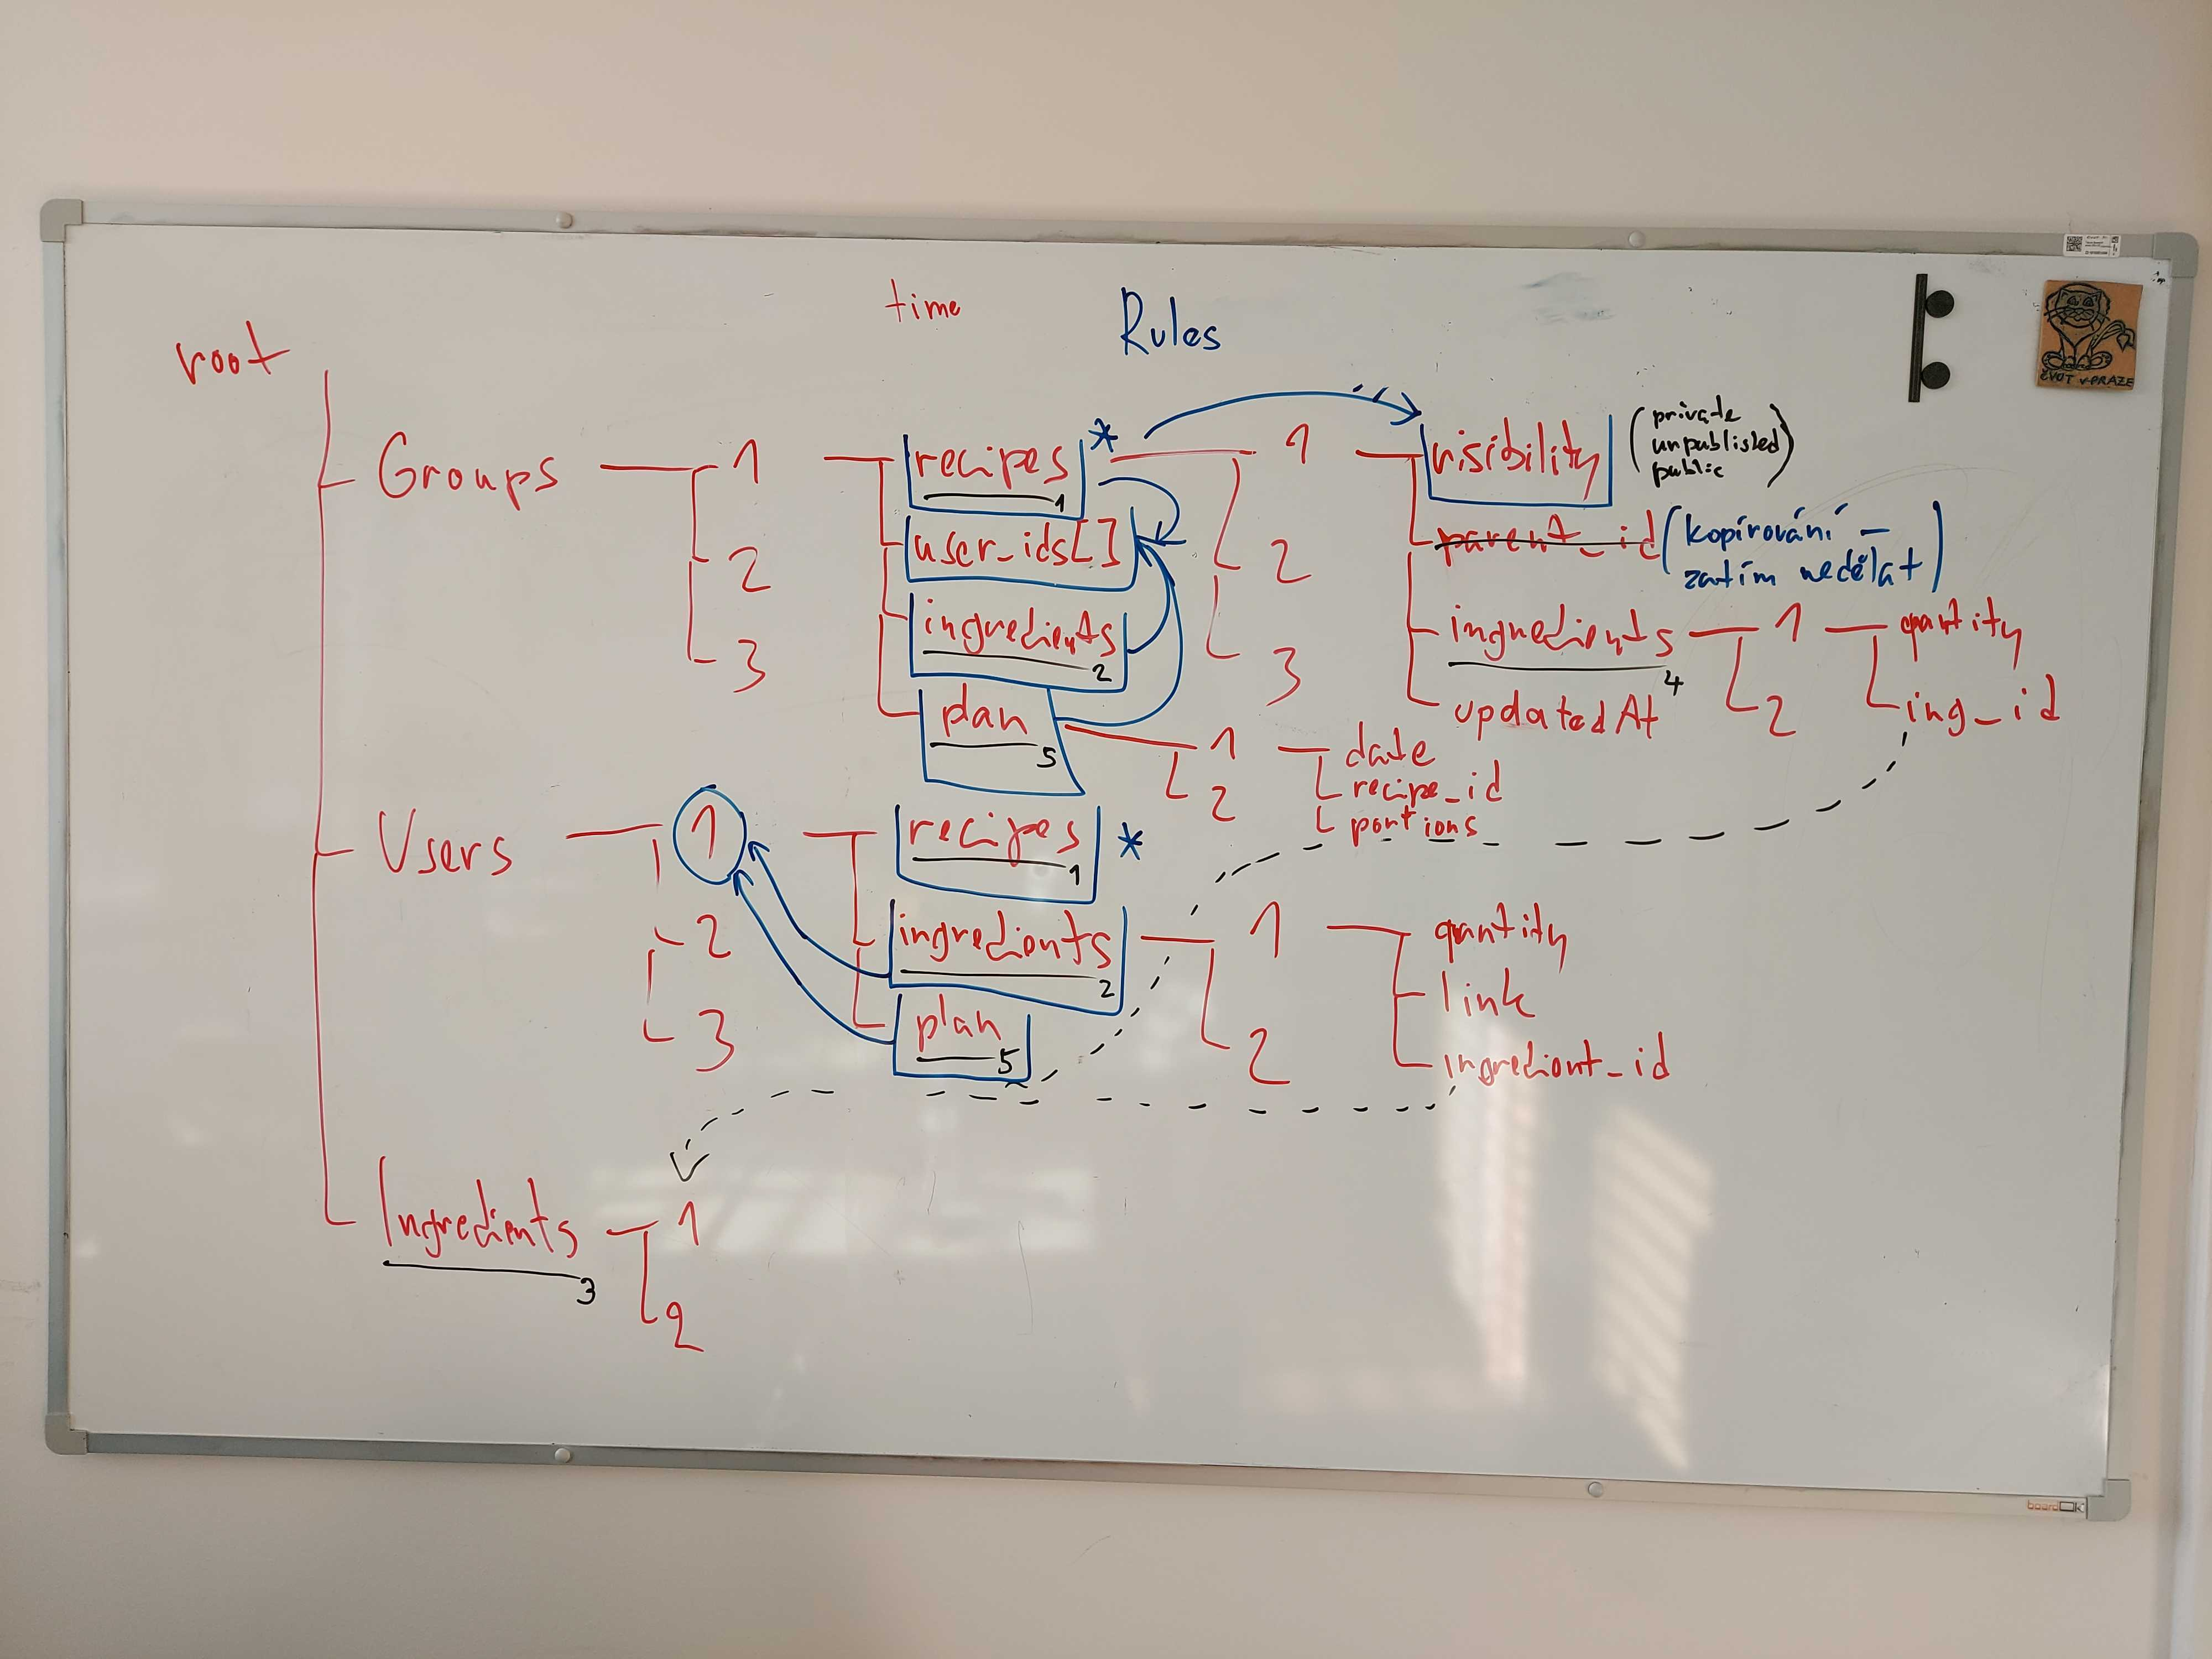
\includegraphics[width=\textwidth]{images/firestore-structure}
    \caption{Struktura dat ve Firestore} \label{picture:recipeo:firestore-structure}
\end{figure}

\section{Uložiště ve Firebase}
Firebase poskytuje i vlastní uložiště dat pod názvem \emph{Cloud Storage}~\cite{CloudStorage}. Zde je potřeba ukládat externí obrázky, které uživatelé
nahrají k receptu či ingredienci. Strukturu složek jsem zde zvolil stejně jako v databázi.

\section{Data v aplikaci}
Kromě uložení dat na serveru je nutné s nimi pracovat také na frontendu. Zde jsem zvolil \emph{Vuex} pro správu dat. Původně
můj návrh počítal s tím, že se data budou stahovat postupně, až když je bude uživatel potřebovat. Fungovalo by to tak, že by
se například na stránce pro recepty zobrazilo 30 receptů a až když by uživatel prošel přes všechny na konec obrazovky, stáhnuly
by se další. S tímto řešením ale nastal problém, protože jsem spoléhal na to, že na fulltextové vyhledávání použiji službu
\emph{Algolia}. Na konec kvůli složitosti řešení a kvůli tomu služba byla nákladná po překročení limitů, jsem tuto možnost zavrhnul.

Zvolil jsem tedy vyhledávání na frontendu, k čemuž je ale potřeba mít všechna data již při startu aplikace. Začal jsem tedy
zkoumat, zda je možné využít cachování a tím zefektivnit čtení z databáze. \emph{Firestore} poskytuje cache již v základu~\cite{FirestoreCache} a bylo
tedy potřeba ji pouze aktivovat.
